\documentclass[11pt,a4paper]{article}
\usepackage{iftex}
\ifPDFTeX
  \usepackage[T1]{fontenc}
  \usepackage[utf8]{inputenc}
  \usepackage{lmodern}
\else
  \usepackage{fontspec}
  \setmainfont{lmroman10-regular.otf}[
    BoldFont=lmroman10-bold.otf,
    ItalicFont=lmroman10-italic.otf,
    BoldItalicFont=lmroman10-bolditalic.otf]
  \setmonofont{lmmono10-regular.otf}
\fi
\usepackage[polish]{babel}
\usepackage[margin=2.2cm]{geometry}
\usepackage{amsmath,amssymb,booktabs,tabularx,graphicx,float,enumitem,microtype}
\usepackage[font=small,labelfont=bf]{caption}
\usepackage{titlesec}
\usepackage[hidelinks]{hyperref}
\graphicspath{{figures/}}
\setlist{nosep,leftmargin=1.5em}
\setlength{\parindent}{0pt}
\setlength{\parskip}{3pt}
\setlength{\intextsep}{6pt}
\titlespacing*{\section}{0pt}{2.2ex}{1ex}
\titlespacing*{\subsection}{0pt}{1.6ex}{0.8ex}
\setlength{\emergencystretch}{1.5em}
\renewcommand{\arraystretch}{1.15}

\begin{document}
\hypersetup{pageanchor=false}
\begin{titlepage}
\centering
{\Large Akademia Górniczo-Hutnicza\par}
\vspace{3.0cm}

\includegraphics[width=0.3\linewidth]{logo.jpg}
\vspace{1.0cm}
\\
{\large Modele Kolejkowe w IT\par}
\vspace{1.2cm}
{\LARGE\bfseries Symulacja stacji ładowania robotów\par}
\vspace{0.6cm}
{\large Model otwarty i model zamknięty\par}
\vspace{2.2cm}
{\large Julia Wiater\par Łukasz Mamczura\par Kacper Wójcik\par}
\vfill
{\large 16.11.2026\par}
\end{titlepage}
\hypersetup{pageanchor=true}
\setcounter{page}{2}

\section{Cele i założenia projektu}
Projekt przedstawia stację, w której kilka robotów korzysta z ograniczonej liczby ładowarek. Gdy wszystkie stanowiska są zajęte, robot czeka w jednej wspólnej kolejce FIFO. Celem jest ocena czasu oczekiwania, wykorzystania stacji i dostępności floty przy różnych liczbach robotów i ładowarek.

Przyjęto następujące uproszczenia:
\begin{itemize}
\item jedna ładowarka obsługuje jednego robota, a rozpoczęte ładowanie trwa do końca;
\item w podstawowych modelach ładowarki mają jednakowe parametry, a czas obsługi jest stały lub wykładniczy;
\item kolejka nie ma limitu pojemności; nie uwzględnia się awarii, dojazdów ani zużycia energii;
\item stacja rozpoczyna pusta, a w modelu zamkniętym wszystkie roboty początkowo pracują.
\end{itemize}

\section{Opis zagadnienia i modele}
Podstawowe oznaczenia parametrów zestawiono w tabeli~\ref{tab:symbols}. Użytkownik podaje liczbę robotów i ładowarek, czas ładowania oraz tempo napływu lub średni czas pracy robota. W silniku czas jest liczony w minutach.
\begin{table}[H]
\centering\small
\begin{tabularx}{\linewidth}{lXl}
\toprule
Symbol & Znaczenie & Jednostka \\
\midrule
$c$, $N$ & Liczba ładowarek i liczba robotów w stałej flocie & szt. \\
$d$, $d_i$ & Stały czas ładowania wspólny lub dla ładowarki $i$ & min \\
$1/\mu$ & Średni czas ładowania przy obsłudze wykładniczej & min \\
$\lambda$ & Intensywność napływu w modelu otwartym & zgłoszenia/h \\
$\alpha$ & Intensywność zgłoszeń jednego pracującego robota & zgłoszenia/h \\
\bottomrule
\end{tabularx}
\caption{Oznaczenia używane w sprawozdaniu.}\label{tab:symbols}
\end{table}

\subsection{Model otwarty}
Robot przybywa z otoczenia, oczekuje, ładuje się i opuszcza model. Napływ jest zawsze Poissona i nie zależy od zajętości stacji. Odstępy między zgłoszeniami są losowane z rozkładu wykładniczego. Przygotowano dwa warianty obsługi:
\begin{itemize}
\item \textbf{M/D/c}: każde ładowanie trwa dokładnie podany czas $d$;
\item \textbf{M/M/c}: czas każdego ładowania jest losowany niezależnie z rozkładu wykładniczego o podanej średniej $1/\mu$.
\end{itemize}
Porównujemy tę samą intensywność napływu i ten sam średni czas obsługi. Wpisane 20 minut oznacza więc stałe 20 minut albo średnią losowanych czasów. Jeżeli przez dłuższy czas napływa więcej robotów, niż stacja może naładować, kolejka rośnie. Krótkie kolejki mogą pojawiać się także wtedy, gdy średnia wydajność stacji jest wystarczająca.

\subsection{Model zamknięty i indywidualna obsługa}
Stała flota $N$ robotów powtarza cykl: praca, kolejka FIFO, ładowanie i powrót do pracy. Czas pracy jest losowany niezależnie z rozkładu wykładniczego. Obsługa może być stała (M/D/c) albo wykładnicza (M/M/c). Są to warianty ze skończonym źródłem: mniej pracujących robotów oznacza mniejszą intensywność kolejnych zgłoszeń. Liczba ładowarek nie przekracza liczby robotów, a do floty nie dochodzą nowi członkowie.

Dodatkowy wariant zamknięty przypisuje każdej ładowarce własny, stały czas $d_i$. Robot z początku kolejki trafia do najszybszej wolnej ładowarki, a remis rozstrzyga niższy numer stanowiska. W eksperymentach wariant z $c$ ładowarkami używa pierwszych $c$ pozycji podanej listy czasów. Jednakowe czasy i ten sam seed dają ten sam przebieg co w podstawowym modelu zamkniętym ze stałą obsługą.

\clearpage
\section{Symulacja i mierzone wielkości}
Silnik zdarzeń dyskretnych przeskakuje do kolejnych przyjść i zakończeń ładowania. Przy remisie najpierw obsługuje zakończenia, potem przyjścia, a na końcu zapisuje próbkę. Statystyki uwzględniają czas spędzony w każdym stanie.

System przy stacji obejmuje kolejkę i ładowarki. Roboty pracujące poza stacją nie są do niego wliczane. Wyniki przedstawiają:
\begin{itemize}
\item \textbf{Średnie liczby robotów w kolejce $Q$ i przy stacji $K$.} Dłużej trwające stany mają większy wpływ na średnią niż krótkie zmiany.
\item \textbf{Średni czas oczekiwania $W$.} Pokazuje, ile czasu robot czeka przed rozpoczęciem ładowania. Nie obejmuje samego ładowania.
\item \textbf{Wykorzystanie ładowarek $u$.} Określa, jaką część dostępnego czasu stanowiska spędziły na ładowaniu.
\item \textbf{Prawdopodobieństwo pustej kolejki i zajętości stanowisk.} Wynika z tego, przez jaką część obserwacji nikt nie czekał lub zajęta była określona liczba ładowarek. Pusta kolejka nie oznacza, że ładowarki są wolne.
\item \textbf{Dostępność floty.} W modelu zamkniętym $E[R]$ to średnia liczba pracujących robotów, a $A$ to ich średni udział w całej flocie, podawany także w procentach.
\end{itemize}
Wykresy chwilowe pokazują stan w danym momencie. Średnie narastające opisują cały czas od początku symulacji. Oczekiwanie jest uwzględniane w średniej dopiero wtedy, gdy robot rozpocznie ładowanie; nadal oczekujące roboty nie są traktowane tak, jakby czekały zero minut.

\section{Aplikacja}
Projekt korzysta z Pythona, Streamlit, Matplotlib i pandas. Po instalacji \texttt{requirements.txt}, z katalogu projektu uruchamiamy:\par
\texttt{python -m streamlit run app.py}.
\begin{itemize}
\item \textbf{Symulacja i wykresy}: parametry, wybór stałej lub wykładniczej obsługi, seed, wyniki, wykresy i eksport CSV/PNG w ZIP.
\item \textbf{Eksperymenty}: listy wartości $c$, $N$ lub $\lambda$ oraz liczba powtórzeń.
\item \textbf{Opis modeli i miar}: założenia i interpretacja wyników.
\end{itemize}
W zamkniętych modelach suwak czasu odczytuje stan i intensywności z zapisanej trajektorii. Wykres czasu pokazuje $W$; czas pobytu w systemie pozostaje w tabeli i eksporcie.
\begin{figure}[H]
\centering
\includegraphics[width=0.75\linewidth,trim=0 0 0 225,clip]{ui.jpg}
\caption{Wyniki w aplikacji dla M/M/c: $c=2$, średnie ładowanie 20 min, $\lambda=4$/h, 24 h, seed 42. To pojedynczy przebieg, a nie średnie z powtórzeń.}\label{fig:ui}
\end{figure}

\clearpage
\section{Eksperymenty symulacyjne}
Każdy wariant badano przez 168 godzin, w pięciu powtórzeniach z seedami od 42 do 46. Tabele podają średnie z powtórzeń, z uwzględnieniem rozruchu od pustej stacji.

\subsection{Rodzaj obsługi i liczba ładowarek}
Dla napływu Poissona $\lambda=4$/h porównano od jednej do trzech ładowarek, ze stałą obsługą 20 min lub wykładniczą o średniej 20 min. Kolumna $\rho$ to stosunek napływu do średniej wydajności.
\begin{table}[H]
\centering\small
% BEGIN GENERATED TABLE: open
\begin{tabular}{lrrrrr}
\toprule
Model & $c$ & $\rho$ & $Q$ & $W\pm s_W$ [min] & $u$ [\%] \\
\midrule
M/D/c & 1 & 1,33 & 71,243 & \(1108,400 \pm 205,404\) & 99,8 \\
M/M/c & 1 & 1,33 & 69,285 & \(1066,535 \pm 313,401\) & 99,6 \\
M/D/c & 2 & 0,67 & 0,475 & \(7,367 \pm 1,747\) & 63,9 \\
M/M/c & 2 & 0,67 & 1,008 & \(15,567 \pm 6,374\) & 64,1 \\
M/D/c & 3 & 0,44 & 0,073 & \(1,133 \pm 0,189\) & 42,6 \\
M/M/c & 3 & 0,44 & 0,151 & \(2,324 \pm 1,200\) & 42,8 \\
\bottomrule
\end{tabular}
% END GENERATED TABLE: open
\caption{Model otwarty. $s_W$ to odchylenie standardowe z pięciu powtórzeń.}\label{tab:open}
\end{table}
Dla $c=1$ napływ przekracza średnią wydajność 3/h, więc wyniki opisują narastającą kolejkę w skończonym czasie. Dla $c=2$ uzyskano $W=7{,}37$ min przy stałej obsłudze i $15{,}57$ min przy wykładniczej. Trzecia ładowarka zmniejszyła te czasy do 1,13 i 2,32 min.

\subsection{Wpływ liczby robotów i ładowarek w zamkniętej flocie}
Porównano $N=10,15,20$ i $c=1,2,3$ dla obu rodzajów obsługi. Średni czas pracy wynosił 120 min, a stały lub średni czas ładowania 20 min. Tabela~\ref{tab:closed} dotyczy $N=10$, a rysunek~\ref{fig:closed} wszystkich flot.
\begin{table}[H]
\centering\small
% BEGIN GENERATED TABLE: closed
\begin{tabular}{lrrrrrr}
\toprule
Model & $c$ & $Q$ & $W$ [min] & $E[R]$ & $u$ [\%] & $A$ [\%] \\
\midrule
M/D/c & 1 & 2,865 & 57,963 & 6,153 & 98,2 & 61,5 \\
M/M/c & 1 & 3,108 & 65,252 & 5,943 & 94,9 & 59,4 \\
M/D/c & 2 & 0,344 & 5,035 & 8,289 & 68,3 & 82,9 \\
M/M/c & 2 & 0,554 & 8,293 & 8,106 & 67,0 & 81,1 \\
M/D/c & 3 & 0,054 & 0,766 & 8,540 & 46,9 & 85,4 \\
M/M/c & 3 & 0,085 & 1,210 & 8,497 & 47,3 & 85,0 \\
\bottomrule
\end{tabular}
% END GENERATED TABLE: closed
\caption{Model zamknięty dla $N=10$. Dostępny robot pracuje poza stacją.}\label{tab:closed}
\end{table}
Dla $c=2$ zmiana obsługi ze stałej na wykładniczą zwiększyła $W$ z 5,04 do 8,29 min.
\begin{figure}[H]
\centering
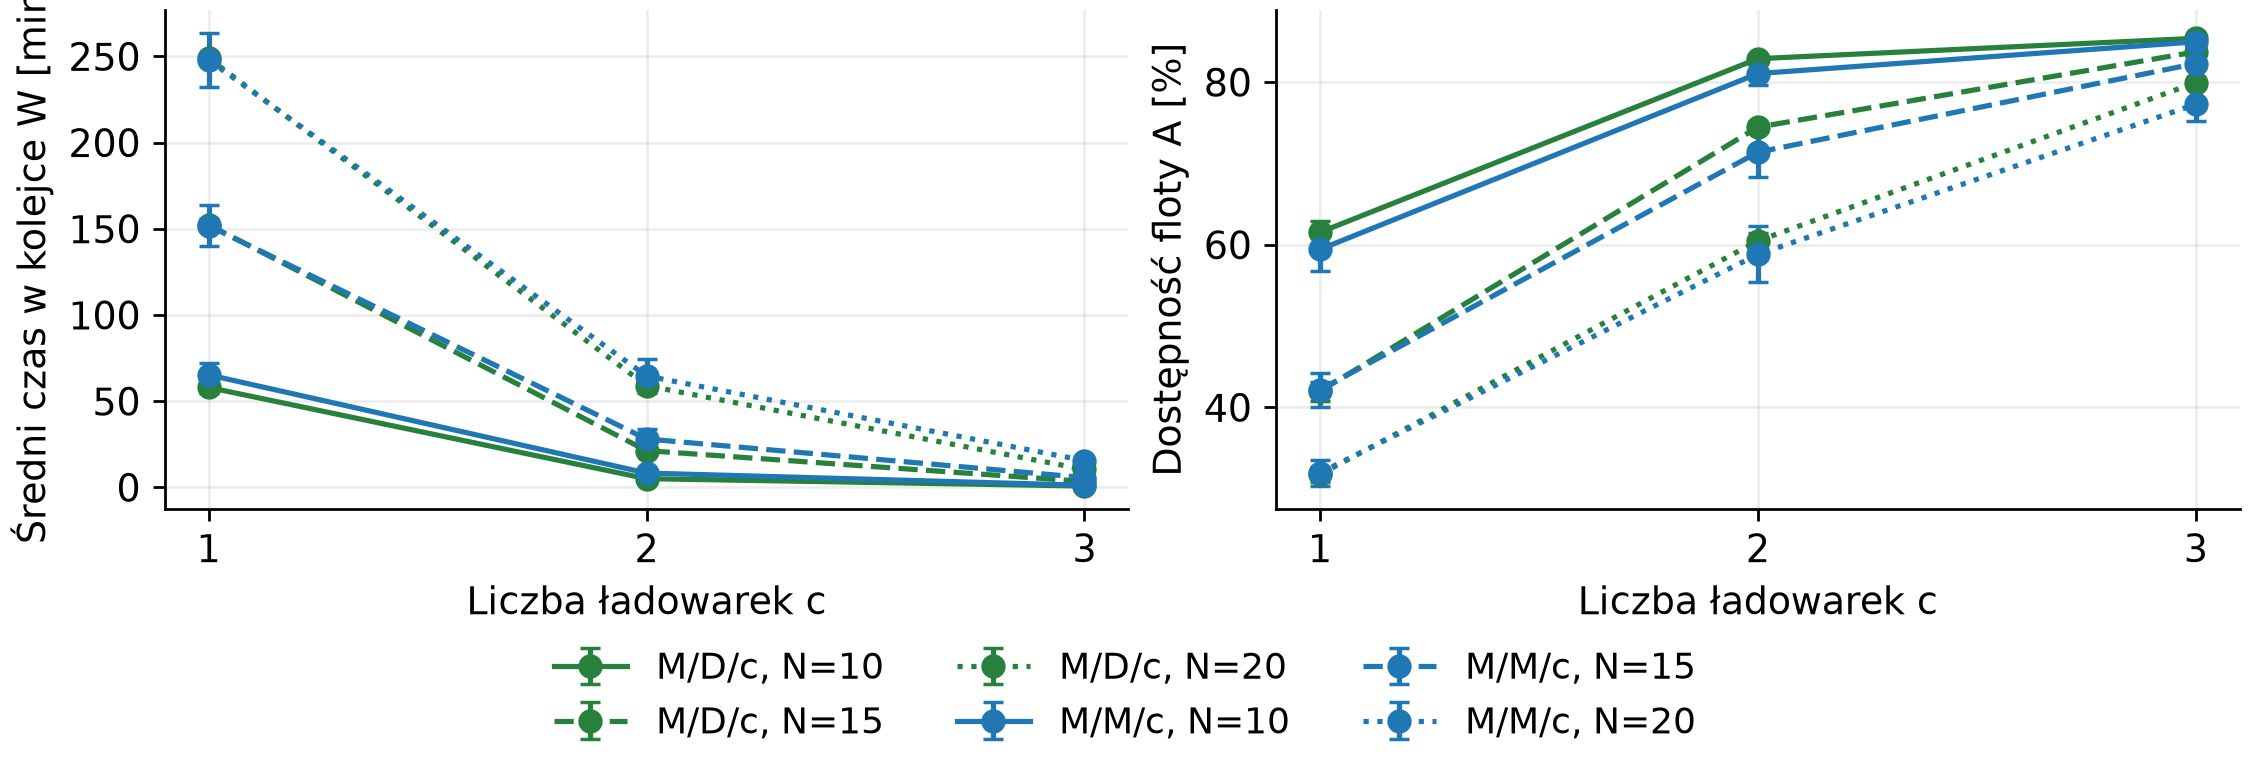
\includegraphics[width=\linewidth]{closed_experiment.png}
\caption{Stała i wykładnicza obsługa. Słupki oznaczają jedno odchylenie standardowe.}\label{fig:closed}
\end{figure}
\clearpage
\subsection{Ładowarki o indywidualnych czasach obsługi}
Dla 10 robotów, dwóch ładowarek i średniego czasu pracy 120 minut porównano cztery konfiguracje. Łączna wydajność w tabeli oznacza liczbę robotów, które stacja może naładować w godzinę, jeżeli wszystkie stanowiska pracują bez przerw.
\begin{table}[H]
\centering\small
% BEGIN GENERATED TABLE: individual
\begin{tabular}{llrrr}
\toprule
Obsługa & $d_1;d_2$ [min] & Wydajność [roboty/h] & $W$ [min] & $A$ [\%] \\
\midrule
Wspólna stała & 20; 20 & 6,0 & 5,035 & 82,9 \\
Indywidualna & 20; 20 & 6,0 & 5,035 & 82,9 \\
Indywidualna & 15; 30 & 6,0 & 5,005 & 83,0 \\
Indywidualna & 10; 30 & 8,0 & 2,151 & 87,5 \\
\bottomrule
\end{tabular}
% END GENERATED TABLE: individual
\caption{Wspólna stała i indywidualna obsługa. Każdy czas $d_i$ jest stały.}\label{tab:individual}
\end{table}
Warianty z czasami 20 i 20 min dały identyczne wyniki. Czasy 15 i 30 min mają tę samą nominalną wydajność 6/h, a uzyskane średnie były zbliżone. Nie ma podstaw, by z tej niewielkiej różnicy wnioskować o przewadze jednego wariantu. Konfiguracja 10 i 30 min skróciła oczekiwanie, ale ma też większą wydajność 8/h. Nie jest to dowód na korzyść samej reguły przydziału.

\subsection{Odczyt stanu i interpretacja wyników}
Przeprowadzono osobny przebieg zamknięty M/D/c dla 10 robotów i dwóch ładowarek. Każde ładowanie trwało 20 minut, średnia praca 120 minut, a czas symulacji 100 minut. Użyto seeda 41. Na końcu czekał jeden robot, dwa były ładowane, a siedem pracowało. Do stacji wpłynęło 11 zgłoszeń, rozpoczęto 10 ładowań i zakończono 8.
\begin{figure}[H]
\centering
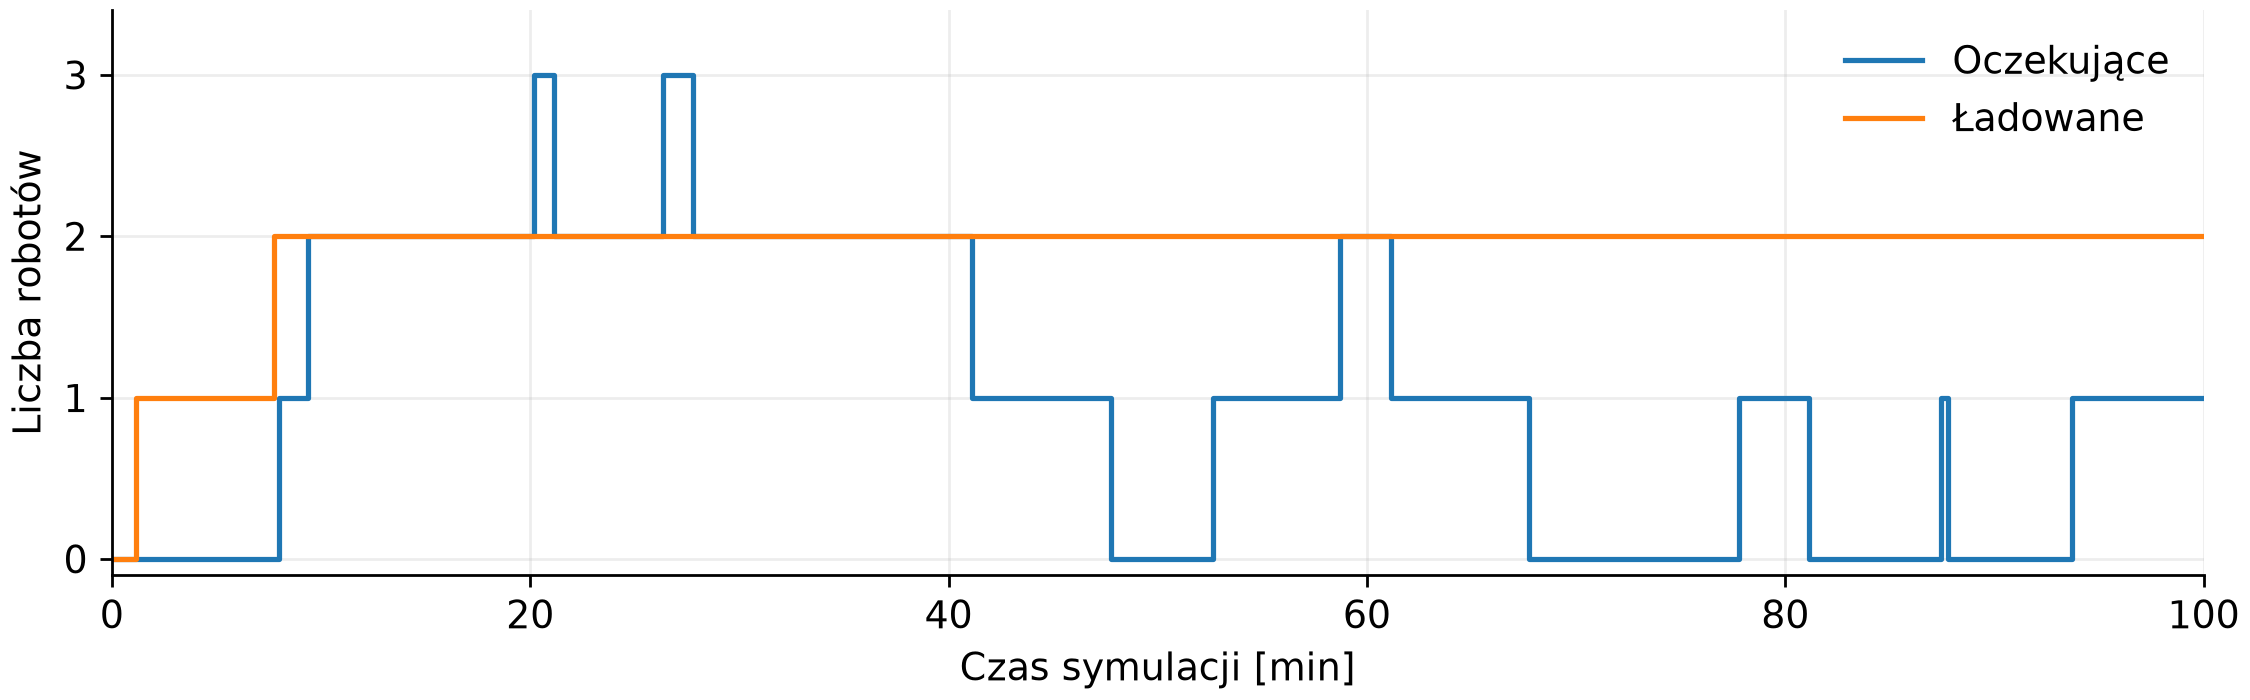
\includegraphics[width=\linewidth]{closed_trace.png}
\caption{Wartości chwilowe dla seeda 41. Po 100 minutach czekał jeden robot, natomiast średnia liczba oczekujących z całego przebiegu wynosiła około 1,014.}\label{fig:trace}
\end{figure}
Tabela intensywności pomaga odróżnić trzy informacje:
\begin{itemize}
\item \textbf{Pojedynczy robot, $\alpha$:} średni czas pracy wynoszący dwie godziny odpowiada 0,5 zgłoszenia na godzinę pracy jednego robota.
\item \textbf{Cała flota w wybranej chwili, $\lambda_n$:} siedem pracujących robotów daje łącznie intensywność 3,5 zgłoszenia na godzinę.
\item \textbf{Napływ zaobserwowany, $\lambda_{\rm obs}$:} w ciągu 100 minut wpłynęło 11 zgłoszeń, co po przeliczeniu daje 6,6 zgłoszenia na godzinę.
\end{itemize}
Średnie oczekiwanie wyniosło około 9,51 minuty i uwzględniało 10 wizyt, które rozpoczęły ładowanie. Średnia liczba pracujących robotów wyniosła około 7,08, co odpowiada dostępności 70,8\%. Wartości te opisują cały przebieg.

\clearpage
\section{Podsumowanie i napotkane trudności}
\textbf{Wnioski z eksperymentów}
\begin{itemize}
\item Dla $N=10$ i stałej obsługi druga ładowarka skróciła oczekiwanie z około 58 do 5 min i zwiększyła dostępność z 61,5\% do 82,9\%. Trzecia przyniosła mniejszą poprawę dostępności. Dobór $c$ wymaga uzgodnienia dopuszczalnego oczekiwania i kosztu stacji.
\item Przy dwóch ładowarkach w obu modelach zaobserwowano dłuższe oczekiwanie dla wykładniczej obsługi niż dla stałej, mimo tej samej średniej. Sama średnia wydajność stacji nie wystarcza do oceny kolejki.
\item W zamkniętej flocie wzrost zajętości stacji ogranicza liczbę pracujących źródeł i dalszy napływ. Nie ma tu jednego zewnętrznego parametru $\lambda$ dla całej floty.
\item W porównaniu ładowarek o różnych czasach trzeba uwzględniać łączną wydajność. Równa liczba stanowisk nie oznacza równej zdolności obsługi.
\end{itemize}


\subsection{Ograniczenia i kierunki rozwoju}
Symulacja kończy się w zadanej chwili, bez opróżnienia kolejki. Długie, jeszcze niezakończone oczekiwania mogą zaniżać obserwowane $W$. Wyniki obejmują rozruch, a pięć powtórzeń pokazuje tylko ograniczony zakres losowej zmienności.

Projekt można rozwinąć o:
\begin{itemize}
\item okres rozgrzewkowy, więcej powtórzeń i przedziały ufności dla wyników;
\item poziom baterii, różne czasy pracy i ładowania, awarie oraz wspólny limit mocy;
\item porównanie reguł wyboru ładowarki przy tej samej wydajności i funkcję kosztu doboru stacji;
\item osobny pomiar prawdopodobieństwa, że liczba pracujących robotów spadnie poniżej ustalonego progu.
\end{itemize}

\end{document}
